% Тут используется класс, установленный на сервере Papeeria. На случай, если
% текст понадобится редактировать где-то в другом месте, рядом лежит файл matmex-diploma-custom.cls
% который в момент своего создания был идентичен классу, установленному на сервере.
% Для того, чтобы им воспользоваться, замените matmex-diploma на matmex-diploma-custom
% Если вы работаете исключительно в Papeeria то мы настоятельно рекомендуем пользоваться
% классом matmex-diploma, поскольку он будет автоматически обновляться по мере внесения корректив
%
\documentclass[14pt]{matmex-diploma}
% \documentclass[14pt]{matmex-diploma-custom}
\usepackage{listings}
\usepackage[numbers]{natbib}
\renewcommand{\baselinestretch}{1.5}
\newfontfamily{\cyrillicfonttt}{Liberation Mono}
\begin{document}
% Год, город, название университета и факультета предопределены,
% но можно и поменять.
% Если англоязычная титульная страница не нужна, то ее можно просто удалить.
\filltitle{ru}{
    chair              = {Кафедра системного программирования},
    title              = {Графическая библиотека на основе PostScript: механизм обработки событий},
    % Здесь указывается тип работы. Возможные значения:
    %   coursework - Курсовая работа
    %   diploma - Диплом специалиста
    %   master - Диплом магистра
    %   bachelor - Диплом бакалавра
    type               = {diploma},
    position           = {студента},
    group              = 544,
    author             = {Макулов Рустам Наилевич},
    supervisorPosition = {к.\,ф.-м.\,н., доц.},
    supervisor         = {Булычев Д.\,Ю.},
    reviewerPosition   = {к.\,ф.-м.\,н., доц.},
    reviewer           = {Кознов Д.\,В.},
    chairHeadPosition  = {д.\,ф.-м.\,н., профессор},
    chairHead          = {Терехов А.\,Н.},
%   university         = {Санкт-Петербургский Государственный Университет},
%   faculty            = {Математико-механический факультет},
%   city               = {Санкт-Петербург},
%   year               = {2013}
}
\filltitle{en}{
    chair              = {Chair of Software Engineering},
    title              = {Event handling in a PostScript-based\\ graphic library},
    author             = {Rustam Makulov},
    supervisorPosition = {},
    supervisor         = {Dmitri Boulytchev},
    reviewerPosition   = {},
    reviewer           = {Dmitry Koznov},
    chairHeadPosition  = {Professor},
    chairHead          = {Andrey Terekhov},
}
\maketitle
\tableofcontents
% У введения нет номера главы
\section*{Введение}
Задача разработки кроссплатформенных программных продуктов может быть решена по-разному. Например, создаются средства и инструменты, которые позволяют использовать один исходный код программ для работы в нескольких средах. Так виртуальная машина Java позволяет запускать программы на языке Java в различных системах, компилируя их в исполняемый код целевой платформы. На сегодняшний день JVM имеет реализации практически для всех операционных систем (ОС). Тем не менее, этого недостаточно для единой кроссплатформенной реализации графических интерфейсов программ, поскольку графическая оболочка конкретной операционной системы занимается отрисовкой примитивов и устанавливает свои ограничения на их поведение. Частично эту проблему решают графические библиотеки, например, Swing \cite{wiki:swing} и Qt \cite{wiki:qt}. Но оконный менеджер, встроенный в графическую оболочку ОС, всё равно регламентирует поведение и внешний вид графических интерфейсов.

Язык PostScript \cite{wiki:plrm} является инструментом для создания высококачественной графики. В качестве графических примитивов в языке выступают отрезки и прямые, которые допускают произвольное масштабирование, вращение и другие преобразования. При этом PostScript является полноценным языком программирования, что, в отличие от декларативных языков, позволяет не только описывать конечное изображение, но и задавать способ его получения.

Значительную роль в графических пользовательских библиотеках играют события --  действия или сигналы, которые могут быть идентифицированы и обработаны программой. В графических приложениях каждое действие пользователя порождает цепочку событий, которые затем обрабатываются в приложении. Взаимодействие объектов также осуществляется при помощи событий: изменение состояния одного объекта приводит к изменению состояния другого, а событие оказывается средством связи между объектами. 

Создание графических интерфейсов с помощью языка PostScript представляется невозможным до тех пор, пока в нем нет событий и механизма для их обработки. Добавление обработки событий позволит создать полноценную графическую библиотеку на PostScript. В свою очередь графическая библиотека на PostScript предоставит возможность создавать приложения, идентичные внешне в различных средах, и задавать новое нестандартное поведение интерфейсов в виде эффектов, например, размытие и волны, не предусмотренные оконным менеджером конкретной ОС и не зависящие от него.

В лаборатории JetBrains математико-механического факультета \sloppy{СПбГУ} был разработан переносимый интерпретатор программ на языке PostScript, исполняемый в среде JVM  \cite{wiki:makulov, wiki:pozdin, wiki:gudiev}. Данный инструмент стал ядром проекта по разработке графической библиотеки на  PostScript. Целью данной работы было расширить язык PostScript путём добавления в него событий и механизма для их корректной обработки. Параллельно в рамках других дипломных работ решались задачи отпимизированной интерпретации путём динамической компиляции, а также реализация графических примитивов и оконного менеджера.

 
\section{Обзор предметной области}

PostScript -- это полнофункциональный язык программирования, спроектированный для создания графических изображений высокого качества. %Виртуальная машина Java  -- это 
Интерпретатор языка PostScript -- это инструмент для исполнения программ на языке PostScript. Он представляет собой JVM-реализацию языка. Swing -- это популярная библиотека для создания графического интерфейса для программ на языке Java. Начиная с версии Java 1.2 (1998 год) Swing включён в Java Runtime Environment. Qt -- это фреймворк для кроссплатформенной разработки на языке программирования C++. 
% При программировании графических интерфейсов пользователя, когда меняется один виджет, часто необходимо уведомить другой виджет. В общем случае необходимо, чтобы для любых объектов была возможность взаимодействовать друг с другом. Например, если пользователь нажимает кнопку закрытия, то должна вызываться функция \texttt{close()}.

Далее будет представлено краткое описание языка PostScript, интерпретатора языка, созданного в лаборатории JetBrains, и механизмов, обеспечивающих взаимодействие объектов в Qt и Swing.


\subsection{PostScript}

Язык PostScript используется для описания графических изображений и текстов с помощью подробных инструкций, отображаемых либо на экране компьютера, либо на печатной странице. В нем есть циклы, файловый ввод/вывод и определения функций. Программы на PostScript представляют собой набор комманд для рисования, выполнение которых позволяет создавать нетривиальные изображения.

Все данные, доступные программам на PostScript, представлены объектами. Операторы языка их создают и используют в качестве аргументов. Каждый объект имеет собственный тип, некоторый атрибут и значение. 
Объекты бывают простые, например: \texttt{boolean, integer, real, name, mark, null} и сложные, например, \texttt{array, dictionary, file, string}.    

Простые объекты являются атомарными: тип, атрибут и значение каждого объекта хранятся вместе, и их нельзя изменить независимо друг от друга. В отличие от значений простых объектов значения сложных объектов лежат в отдельной области памяти. Это позволяет во время копирования сложного объекта не дублировать, а просто передавать ссылку на значение исходного объекта. В результате объекты разделяют одно значение.

Специальная область памяти для хранения значений сложных объектов называется виртуальной памятью. Пространство виртуальной памяти, над которой работают операторы \texttt{save} и \texttt{ restore}, называется локальной памятью. Оно используется для хранения информации, которая требуется в определенный период исполнения. Оставшееся пространство виртуальной памяти, необходимое для хранения информации, время жизни которой не зависит от хода программы, называется глобальной памятью.

Если значения объектов хранятся в них самих или в виртуальной памяти, то сами объекты хранятся на стеках. Всего среда исполнения использует пять стеков: стек операндов, стек словарей, стек исполнения, стек графических состояний, стек ограничивающих изображение путей. Стек исполнения хранит объекты, которые находятся в стадии исполнения. В любой точке исполнения программы он представляет собой стек вызовов программы.

Операторы \texttt{save} и \texttt{ restore} используются для сохранения и восстановления значений объектов в локальной памяти. Первый из них сохраняет состояние локальной памяти и возвращает сохранённое состояние, а второй -- восстанавливает  состояние локальной памяти к состоянию, сохранённому предшествующим оператором \texttt{save}.


Построение рисунка выполняется с помощью графических операторов, например, таких как \texttt{rlineto, stroke, fill}. Результат построения становится видимым на экране после выполнения оператора \texttt{showpage}. Интерпретатор выполняет программу на PostScript и отображает картинку в отдельном окне. После этого изменить получившееся изображение нельзя, потому что в языке отсутствуют поддержка взаимодействия пользователя и программы.

% \subsection{JVM}

% Виртуальная машина Java является платформой для интерпретации байт-кода. Её реализации доступны для многих аппаратных и программных платформ, что позволяет использовать один байт-код для разных платформ, и таким образом создавать универсальные программы. Это явилось одной из причин, почему многие языки програмирования имеют JVM-реализации.



\subsection{Интерпретатор языка PostScript}

В 2013-2014 гг. в рамках проекта лаборатории JetBrains на основе спецификации языка PostScript был создан кроссплатформенный интерпретатор данного языка. Исходный код написан на языке Java, графическая часть была реализована с использованием библиотеки Swing, входящей в Java Runtime Environment.

Не вдаваясь в подробности, можно сказать, что проект состоял из трёх частей: библиотеки общей поддержки времени исполнения, библиотеки графической части и архитектуры, определяющей внутреннюю структуру и задающей связи между основными компонентами. 

Промышленный интерпретатор ghostscript \cite{wiki:ghostscript}, написанный на языке C++, использовался в качестве эталонного интерпретатора.  Его разработка продолжается по настоящее время.


\subsection{Обработка событий в Swing}

События -- это важная часть в любой программе, использующей пользовательский интерфейс. Все подобные приложения управляются событиями. Приложение реагирует на различные типы событий, которые генерируются в процессе его работы. В любой модели событий присутствуют три основные компоненты: источник, приёмник и слушатель (listener). 

Источник события -- это объект, состояние которого подвергается воздействию пользователя или из других объектов. В результате подобного взаимодействия генерируется событие, заключающее в себе изменение состояния в источнике. Слушатель события -- это объект, который уведомляется об изменении состояния. Источник события делегирует задачу обработки события своему слушателю.

Swing обеспечивают взаимодействие между объектами с помощью функций обратного вызова. Обратный вызов -- это указатель на функцию. Таким образом, если необходим вызов функции обработки, чтобы уведомить о некотором событии, передается указатель на другую функцию (обратный вызов) функции обработки. Функция обработки вызовет функцию обратного вызова, когда это необходимо.

Когда в пользовательском интерфейсе что-то происходит, например, нажатие на кнопку или выбор элемента из списка, генерируется событие. Существует несколько типов событий, например, события действия, события текста, события переключения фокуса. События хранят информацию о произошедшем действии, например, если нажата кнопка, то информация об этом -- это время, порядковый номер в списке графических элементов, источник события и изменённые ключи.

Обработка событий в Swing может быть реализована либо с использованием анонимных классов, либо внутренних классов, либо наследуемых классов.


\subsection{Обработка событий в Qt}

В Qt используется альтернатива техники обратного вызова: сигналы и слоты. Сигнал генерируется, когда происходит определённое событие. Виджеты Qt имеют множество определённых заранее сигналов, но всегда можно выделить подкласс виджетов, чтобы добавить свои сигналы на них. Слот -- это функция, которая вызывается в ответ на определенный сигнал. Виджеты Qt имеют множество предопределённых слотов, но обычно выделяют подклассы виджетов и добавляют свои слоты для того, чтобы обрабатывать сигналы, в которых заинтересован разработчик.

Важным моментом является то, что события обрабатываются не мгновенно после возникновения; вместо этого они попадают в очередь событий, получают приоритеты и последовательно обрабатываются. Всем этим процессом управляет диспетчер событий. Диспетчер циклически обрабатывает очередь и отправляет события по месту назначения.%, поэтому это называется циклом обработки событий. 




% while (is_active)
% {
%  while (!event_queue_is_empty)
%  dispatch_next_event();
 
% wait_for_more_events();
% }

% https://wiki.qt.io/Threads_Events_QObjects_Russian

% Основной графический элемент -- это сцена, на которую добавляются графические объекты.




\section{Механизм обработки событий}

Поскольку язык PostScript изначально проектировался с целью описания графики, то в нем отсутствует обратная связь и, следовательно, какой бы то ни был механизм обработки событий.

\subsection{Передача событий из Java в PostScript}

Благодаря тому, что интерпретатор написан на Java, есть возможность обрабатывать события средствами Java: с помощью слушателей событий мыши и клавиатуры. На рис. 1 изображена диаграмма последовательности, на которой изображена передача событий из Java в PostScript.

\begin{figure}[h!]
\label{разрыв_функции}
\centering
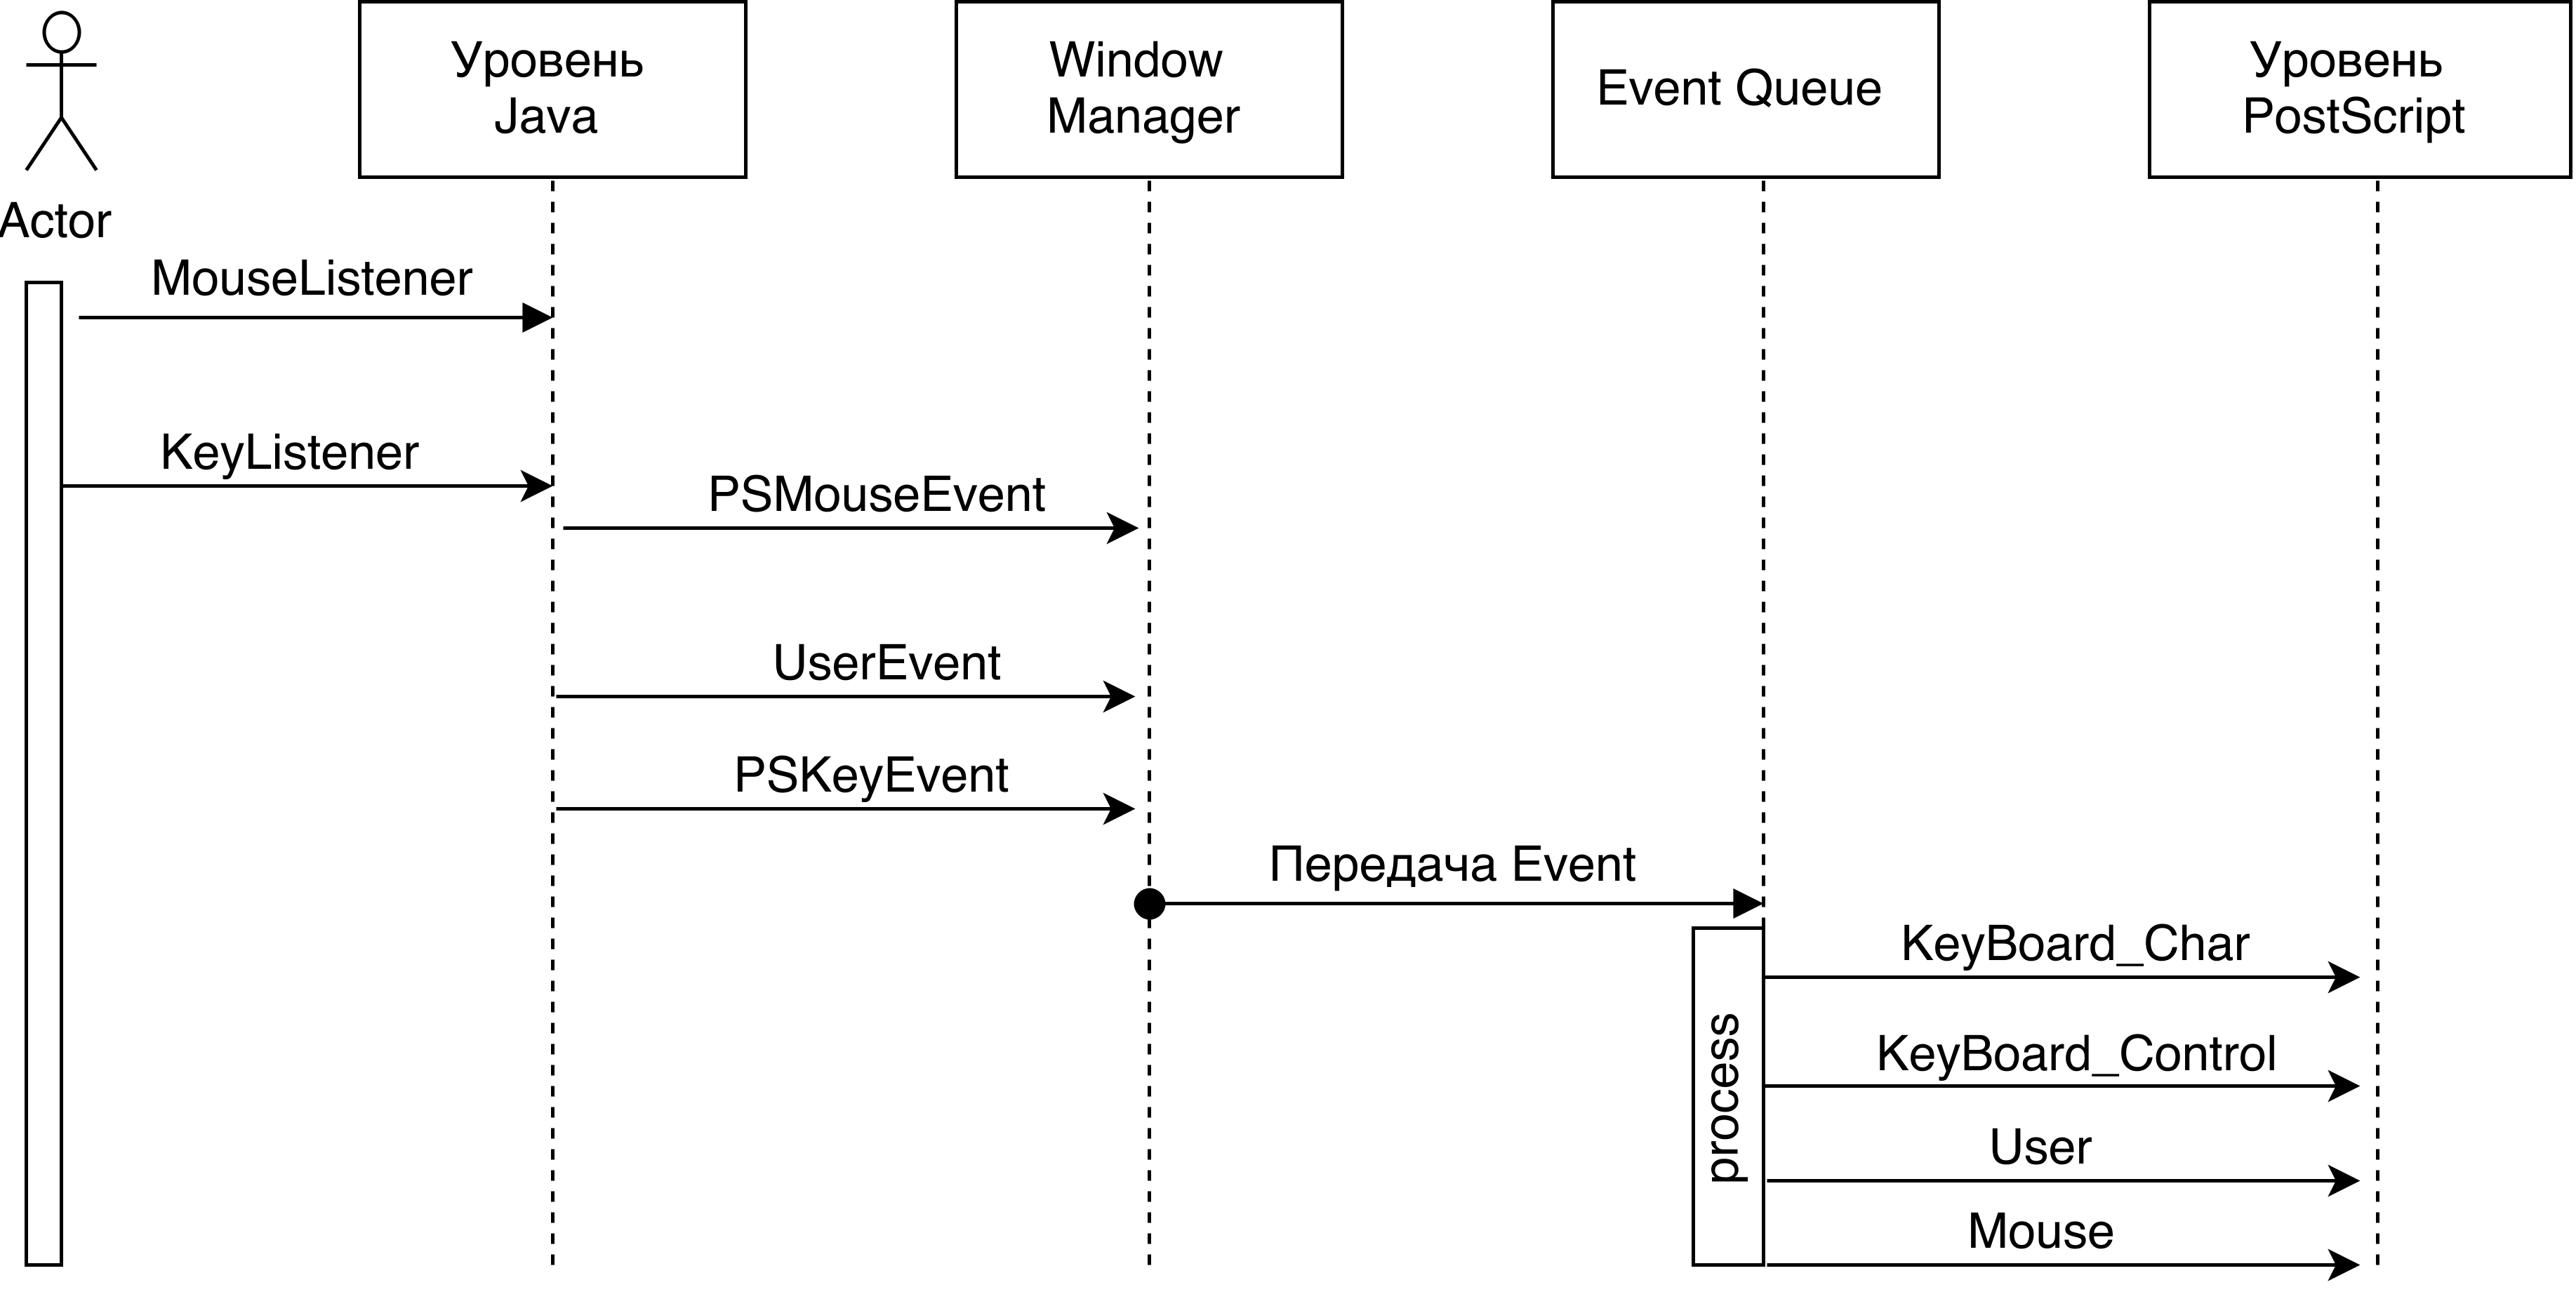
\includegraphics[width=\linewidth,keepaspectratio]{Java_to_PostScript.png}
\caption{Передача событий из Java в PostScript}
\end{figure}

% \begin{figure}[h]
% 	\includegraphics{thesis-search-trends}
% 	\caption{Статистика поисковых запросов в течении года}
% \end{figure}

На уровне Java слушатели мыши и клавиатуры отслеживают действия пользователя и генерируют события трёх типов: PSMouseEvent, UserEvent и PSKeyEvent. Затем эти события с соответствующей информацией передаются в оконный менеджер. Оконный менеджер добавляет полученное событие в очередь обработки событий, и она последовательно исполняет события, поочерёдно вызывая операторы для каждого типа. На уровне PostScript события делятся на следующие типы: ввод печатаемого символа  (\texttt{KEYBOARD\_CHAR}), ввод управляющего символа (\texttt{KEYBOARD\_CONTROL}), действие пользователя (\texttt{USER}) и действие мыши (\texttt{MOUSE}).

Абстрактный класс \texttt{Event} представляет собой события в PostScript, служит родителем для классов \texttt{PSKeyEvent}, \texttt{PSMouseEvent}, \texttt{UserEvent} и содержит в себе тип события \texttt{EventType} (см. рис. 2). В настоящее время реализована поддержка следующих типов событий: \texttt{CLICK, DOUBLE\_CLICK, RELEASE, PRESS, RESIZE, MOVE, DRAG, CLOSE, ENTER, EXIT, RIGHT\_CLICK, PAINT, KEYBOARD\_CHAR, USER, UPDATE\_VALUE, KEYBOARD\_CONTROL}. Класс \texttt{PSKeyEvent} дополнительно содержит код нажатого символа, а \texttt{PSMouseEvent} -- координаты клика. Класс \texttt{UserEvent} содержит строку -- команду и предназначен для реализации механизма обратной связи: из PostScript в Java.  Обработка событий мыши и клавиатуры производится в операторах \texttt{keyevent} и \texttt{mouseevent}. В результате работы этих операторов на стеке исполнения появляется процедура, задаваемая при описании события на уровне PostScript.
% Event, KeyEvent (keyEvent.ps, keyCodes.ps), MouseEvent(mouseEvent.ps), EventType
% EventQueueItem, EventQueue

\begin{figure}[h!]
\label{разрыв_функции}
\centering
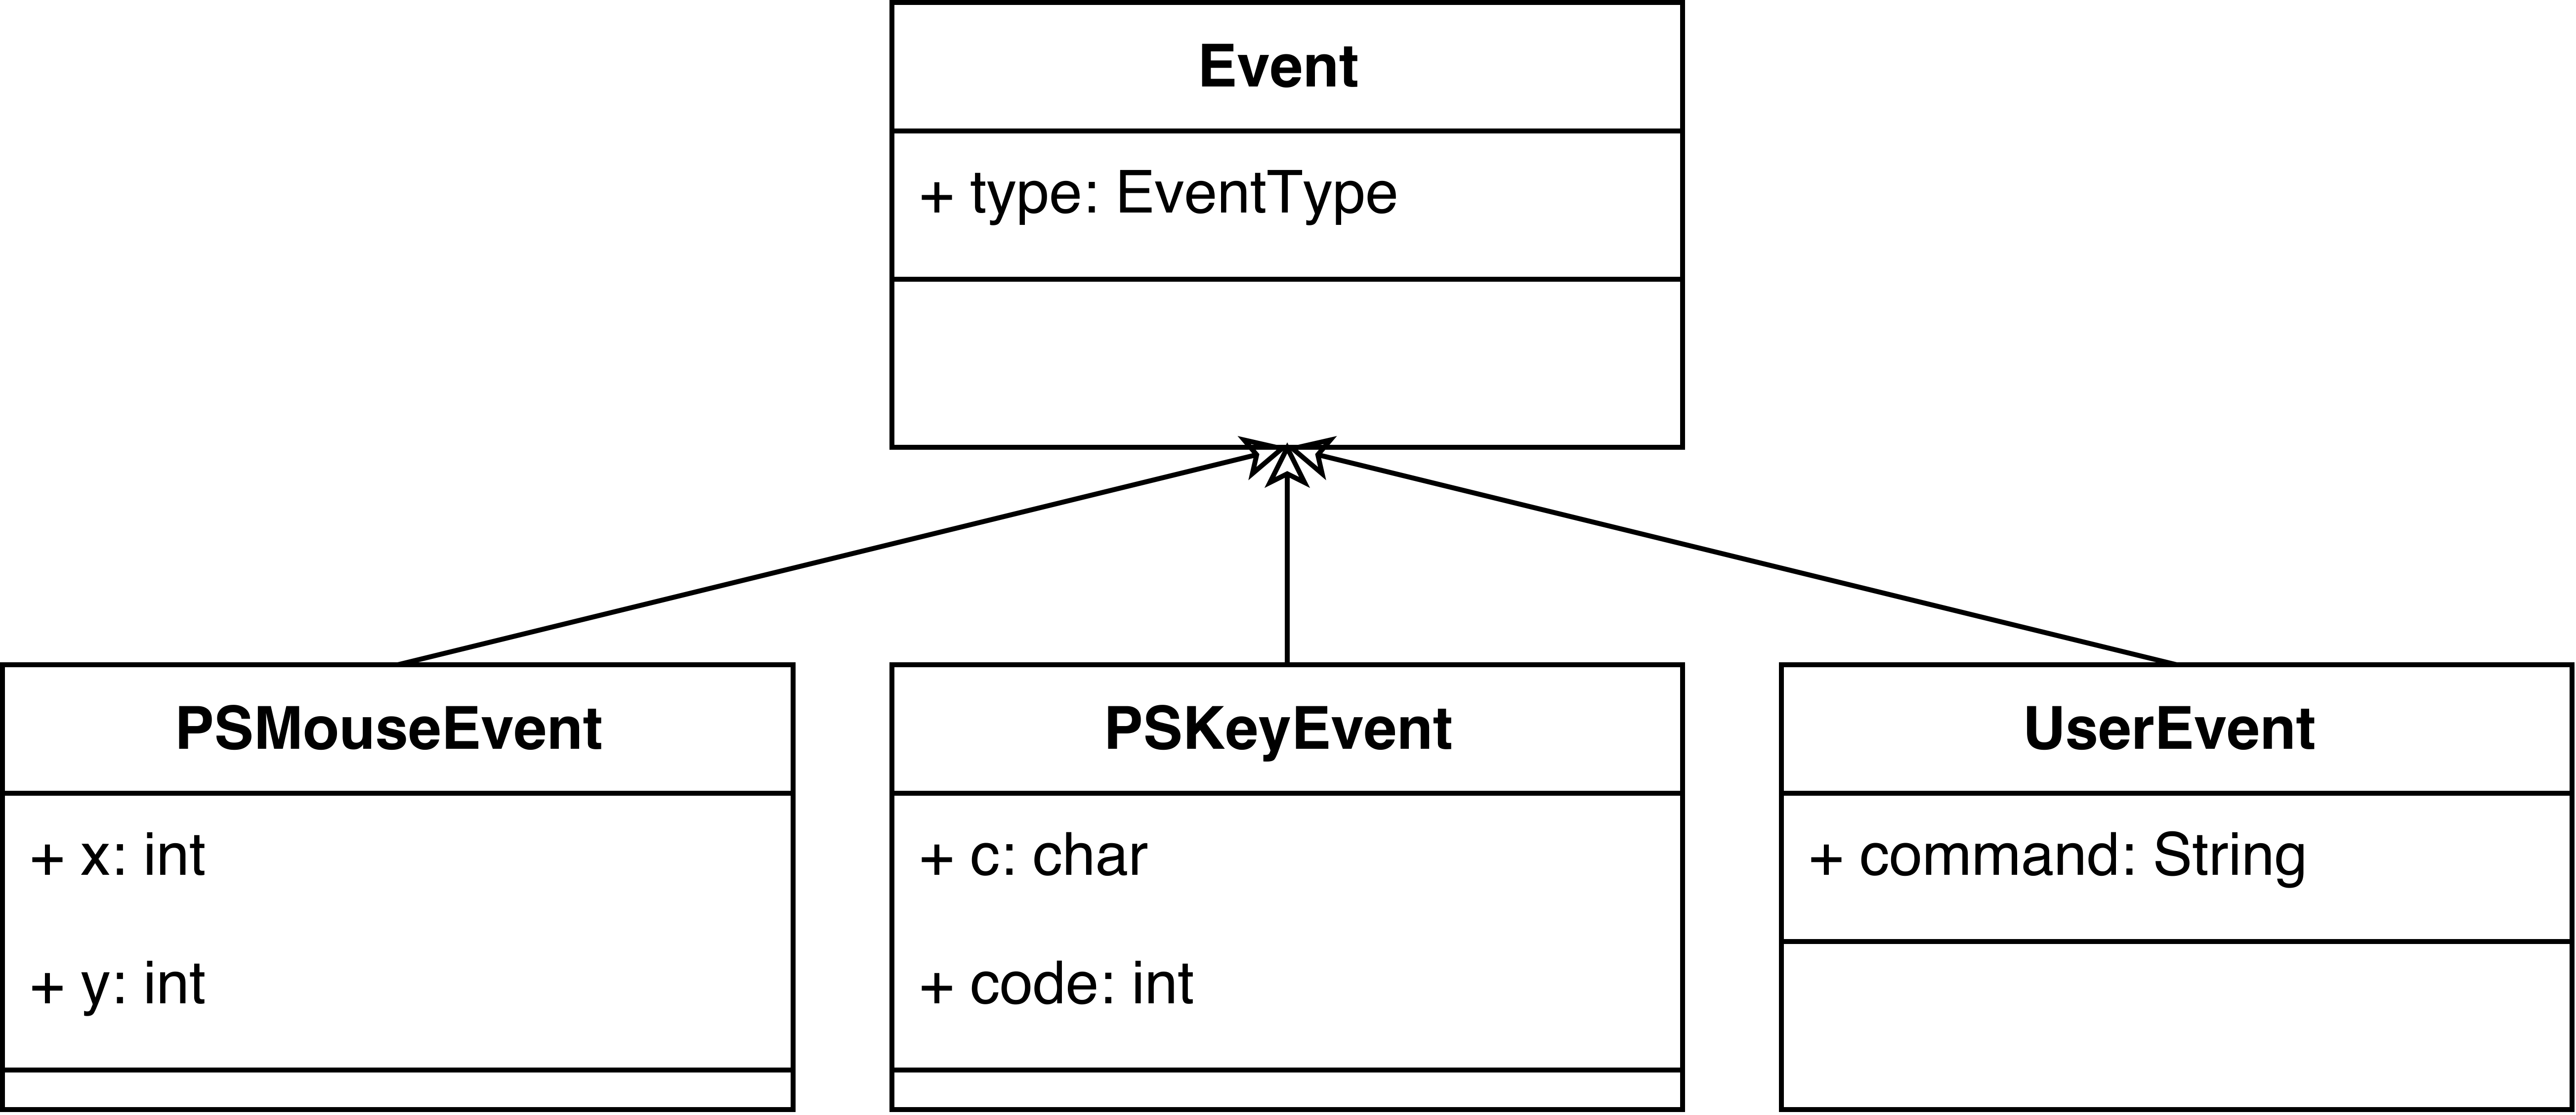
\includegraphics[width=15cm]{Events_from_Java.png}
\caption{Типы событий, передаваемых из Java в PostScript}
\end{figure}


\subsection{Передача событий из PostScript в Java}

Графическую библиотеку предполагается использовать с помощью интерфейса программирования приложений (application programming interface). Для апробации библиотеки был выбран язык Java. С этой целью для каждого графического элемента в PostScript были созданы соответствующие классы на Java, например, \texttt{PSButton}, \texttt{PSWindow} и так далее.

Главный класс, от которого наследуются все элементы графического интерфейса называется \texttt{PSComponent}. На рис. 3 изображена его структура.

\begin{figure}[h]
\label{разрыв_функции}
\centering
% 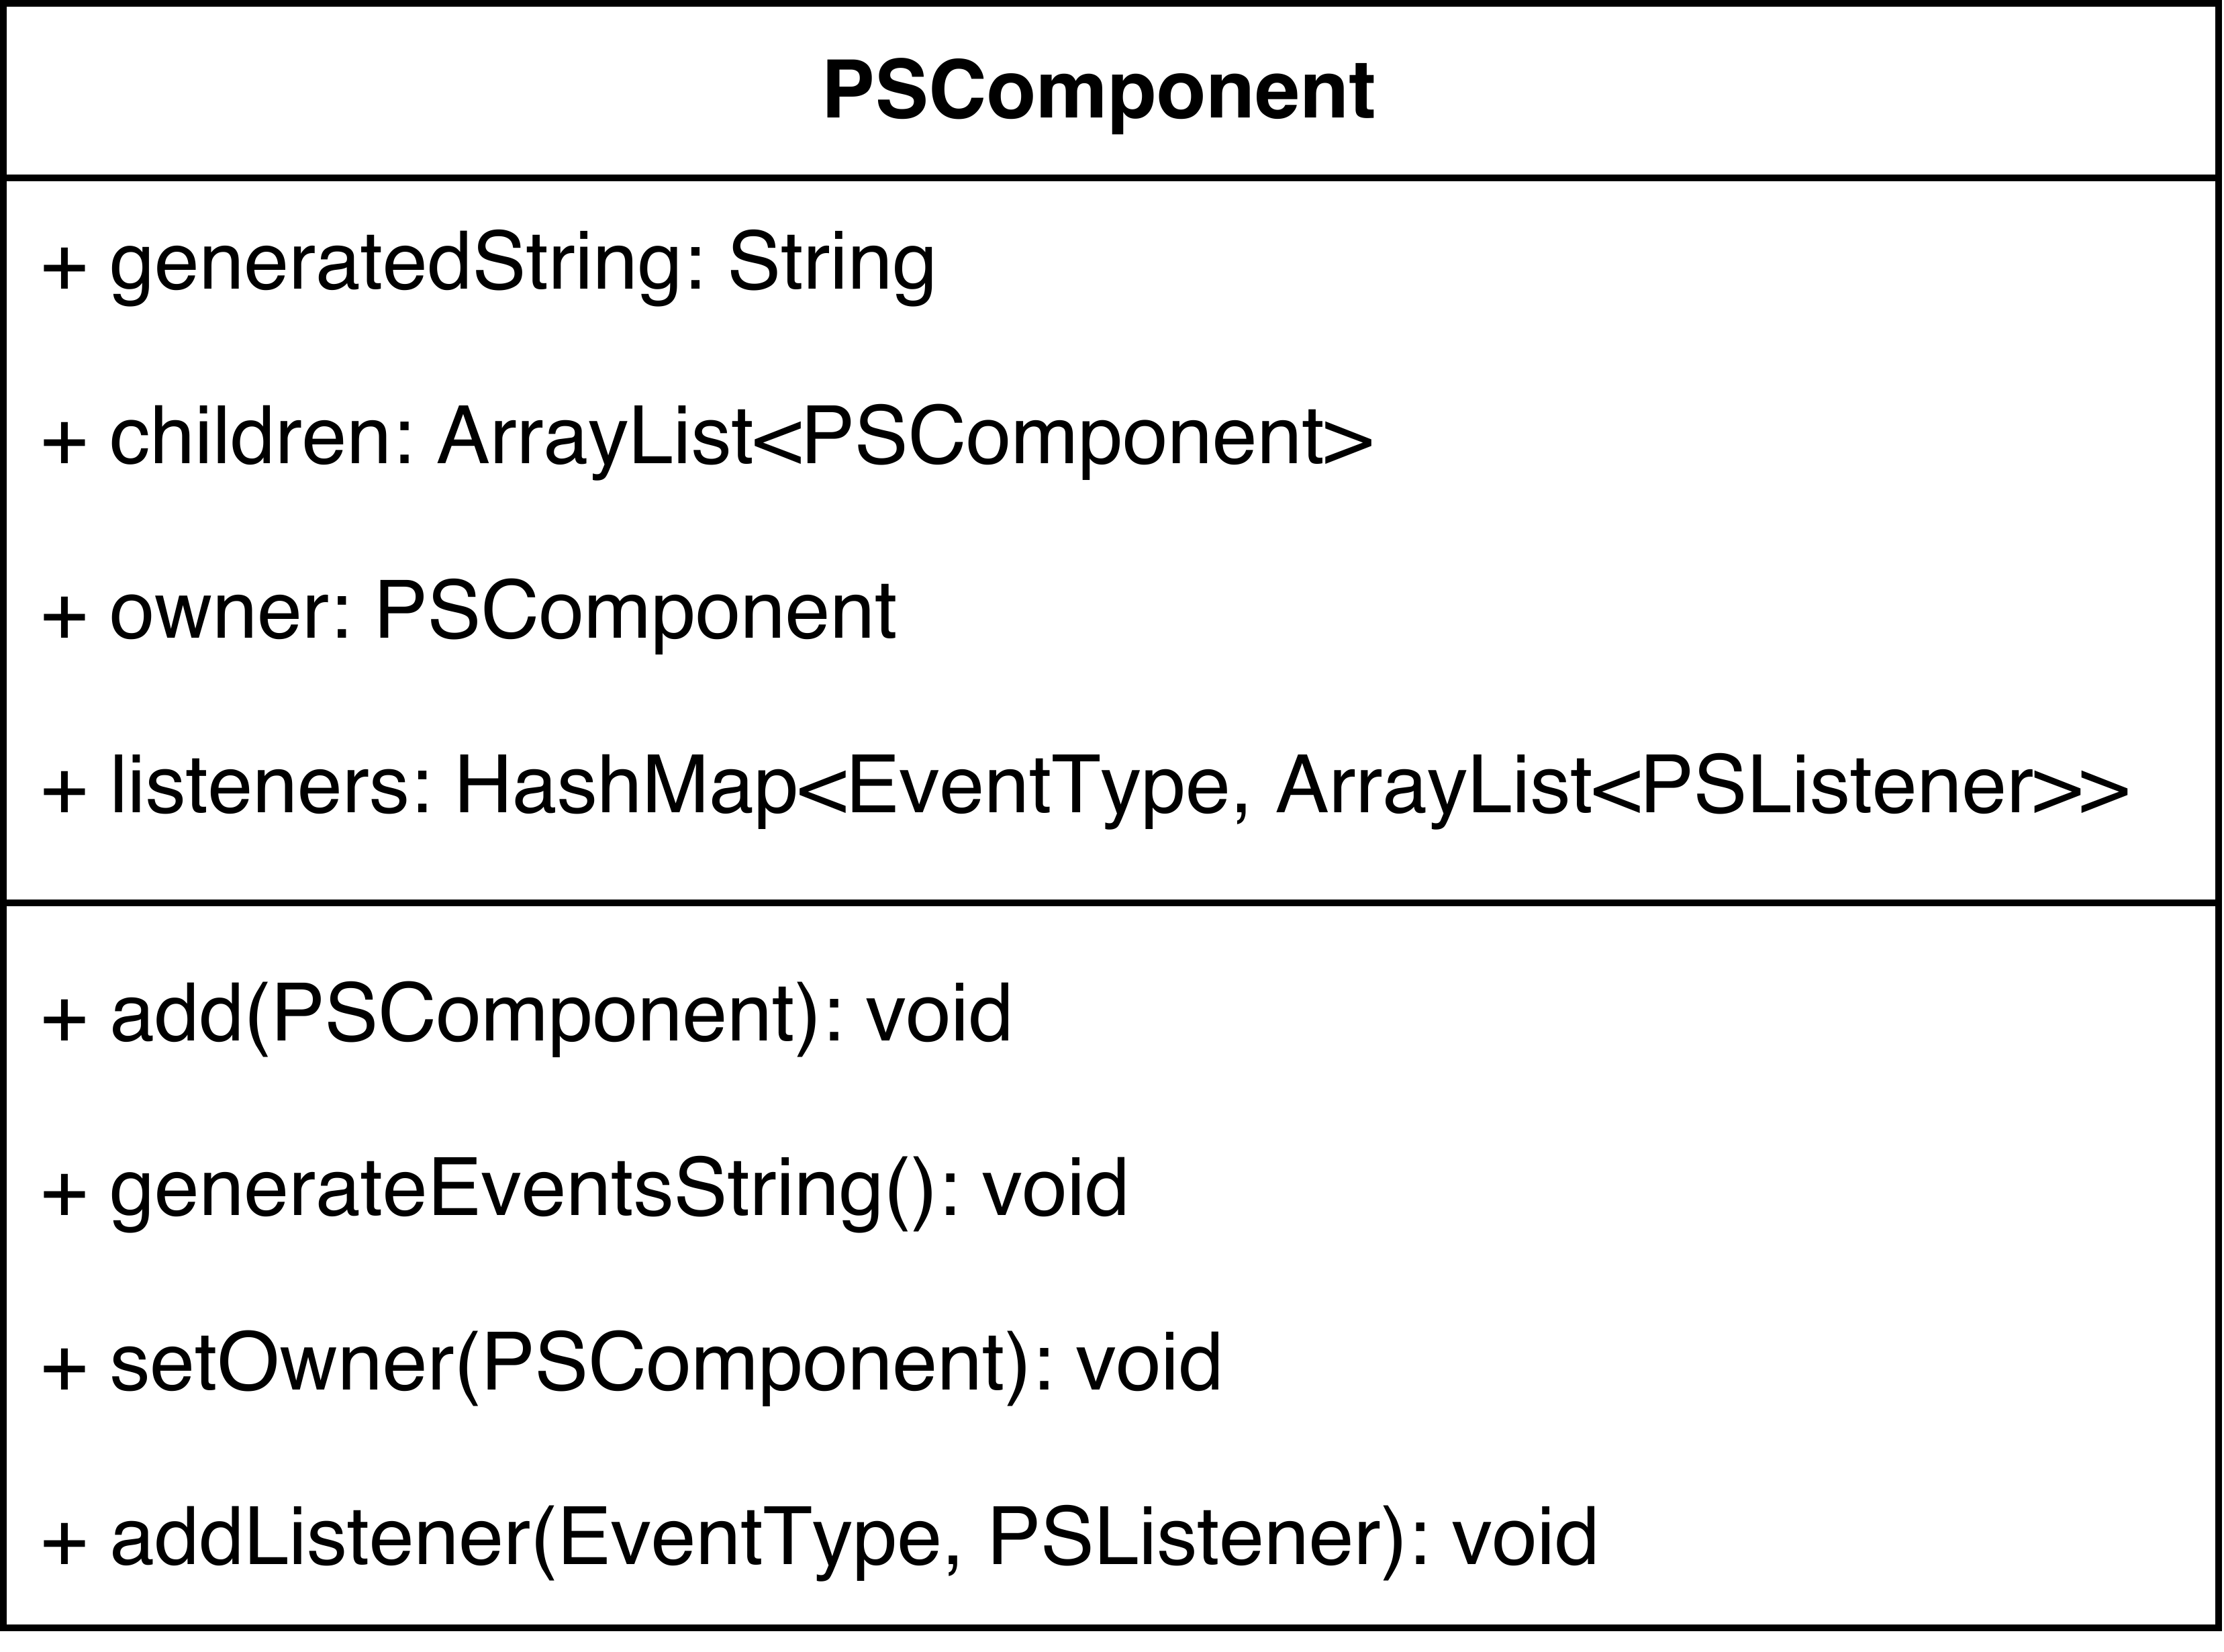
\includegraphics[width=15cm,height=15cm,keepaspectratio]{PSComponent_structure.png}
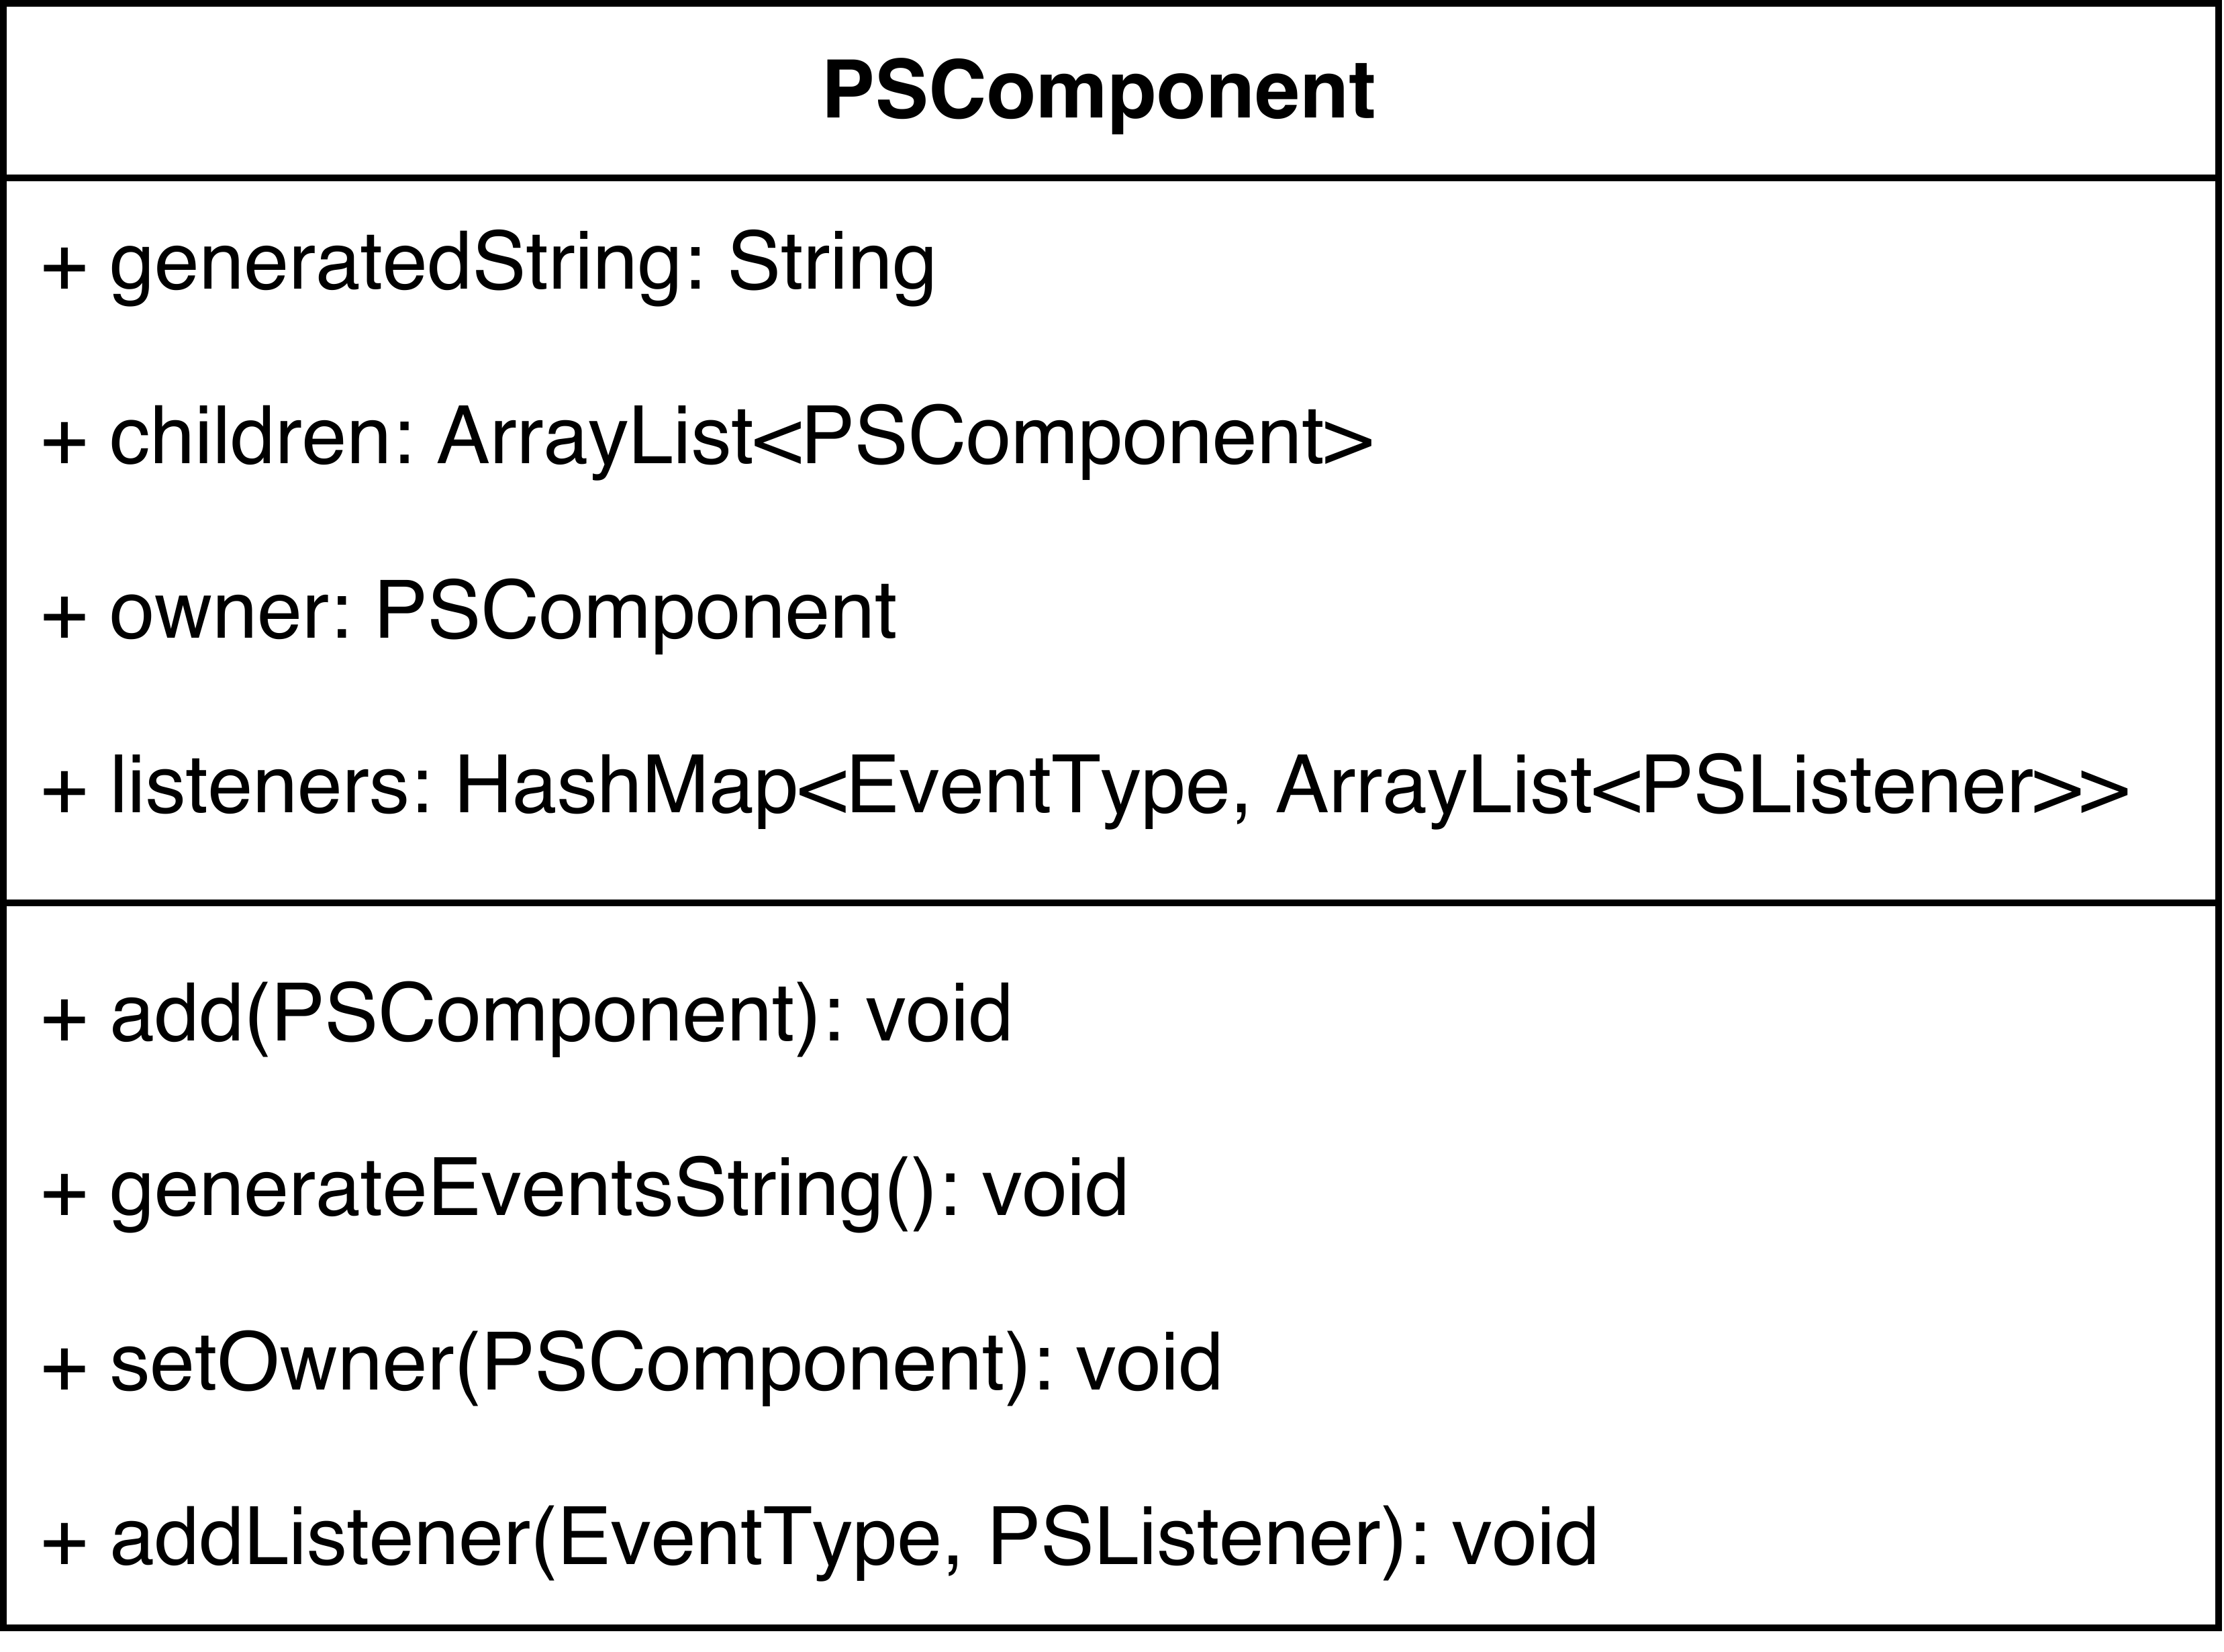
\includegraphics[height=8cm]{PSComponent_structure.png}
\caption{Класс PSComponent}
\end{figure}


Поле \texttt{generatedString} представляет собой фрагмент программы на PostScript и отвечает за добавление компоненты в интерфейс. При этом данный фрагмент собиратся последовательно в несколько этапов. Первоначально он представляет собой шаблон, в который подставляются необходимые значения. Например, для кнопок он имеет следующий вид:\\

\lstset{language=Java,basicstyle=\footnotesize\ttfamily} 
\begin{lstlisting}[frame=single]
%s %d %d %d %d (%s) scene events button
\end{lstlisting}\\

За несколько этапов в шаблон заполняется имя, состоящее из уникального номера и префикса, например, \texttt{window1} для окна и \texttt{button2} для кнопки. Далее идут координаты левого нижнего угла, размеры по горизонтали и вертикали, надпись на кнопке (строки на PostScript указываются в скобках). Затем указывается имя родительского элемента, к которому прикрепляется элемент (по умолчанию это сцена (scene)). Ключевое слово \texttt{button}, необходимое для завершения создания кнопки.

Передача информации в обратную сторону, то есть из PostScript в Java была выполнена динамически, а именно, в тот момент когда добавляется слушатель на Java, как в данном примере \\


\lstset{language=Java,basicstyle=\footnotesize\ttfamily} 
\begin{lstlisting}[frame=single]
PSButton psButton = new PSButton(150, 150, 40, 30, "close");
psButton.addListener(EventType evType, PSListener listener){..}
\end{lstlisting}\\

неявно происходит добавление закладки -- слушателя в поле \texttt{listeners}. Во время генерации конечной программы на PostScript, происходит вставка оператора \texttt{sendEventToJava}, отправляющего события на уровне PostScript. Данный оператор в качестве параметров принимает словарь и тип события. Словарь, который содержит в себе всю информацию об элементе графического интерфейса, передаётся автоматически во время исполнения.

Отдельный класс \texttt{Slots} хранит информацию об объектах в PostScript. Она представляет объект класса HashMap. Паре из имени объекта и типа события соответствует процедура или действие, которое задано пользователем на языке Java при инициализации. 


Каждому графическому объекту в PostScript соответствует объект Java. По сути происходит генерация программы на PostScript: каждый такой объект содержит строку-конструктор или команду, при выполнении которой мы получаем нужный элемент графического интерфейса. Команда передается в классе \texttt{UserEvent} в поле \texttt{command}. Данный класс содержит уникальный номер и префикс графического элемента, конкатенация которых в обратном порядке и есть имя объекта (которое теперь содержится внутри каждого), процедура, исполняемая при нажатии, родительский графический компонент.

% Для хранения пользовательских действий привязанных к опеределённому графическому объекту используются слоты. Они представляют объект класса HashMap, который сопоставляет паре из имени объекта и типу события список действий.
% При добавлении слота происходит неявная генерация процедуры, исполняемой при нажатии. При создании кнопки и других элементов интерфейса в PostScript описываются процедуры и типы событий, на которые они должны реагировать. Происходит генерация строки из типа, который потом облегчает поиск в HashMap, и информации, посылаемой оператором \texttt{sendSignalToJava}.

% Самое интересное - это то, как генерируются вот эти самые процедуры. Потому что для каждого элемента интерфейса нужно передавать различную информацию: для кнопки -- это только информация о клике, но для выпадающего списка -- это выбранный элемент и так далее. Эта информация передается в классе PSEvent.


\section{Расширение языка PostScript}
В стандартной реализации языка PostScript отсутствуют функциональные средства, наличие которых необходимо в библиотеке для создания пользовательских интерфейсов, например, события, которые поступают от мыши и клавиатуры, и их обработчики. В связи с этим возникла потребность расширить язык PostScript, добавив в него новые операторы. Это возможно благодаря тому, что интерпретатор, используемый в данном проекте, можно модифицировать в соответствии с возникающими потребностями. Модификация интерпретатора возможна, поскольку он проектировался и создавался  участниками проекта.

Добавление новых функциональных возможностей в PostScript потребовало соответствующего расширения языка и реализующего его интерпретатора. 

\subsection{Добавление событий}
Отслеживание событий в языке было выполнено средствами Java. Для обработки событий используются специальные синтаксические конструкции при создании каждого графического примитива. Графические примитивы -- это кнопки, выпадающие списки, метки и так далее. Например, сигнатура метода, добавляющего кнопку, выглядит следующим образом:\\

\lstset{language=PostScript,basicstyle=\footnotesize\ttfamily} 
\begin{lstlisting}[frame=single]
450 600 100 70 (close)  window1 <</CLICK [{pop quit}[]] >>  button pop
\end{lstlisting}

В двойных угловых скобках передается словарь: пары из типов обрабатываемых событий и ассоциированных с ними процедур. Процедура может быть не одна, а целый список, поэтому также в язык были добавлены списки, отсутствующие в нем. Реализация списков выполнена подобным образом, как реализованы списки на haskell. 

\subsection{Добавление потока}
 Для возможности выполнения графических эффектов был введен оператор \texttt{newThread}. Он используется для создания нового потока с новым контекстом в расширенном PostScript. В качестве входных параметров он использует исполняемые процедуры и число -- количество операндов, которые нужно переместить на стек операндов в новом контексте из стека операндов контекста, в котором оператор был вызван. В самом конце происходит запуск нового потока с процедурой в получившемся контексте. По завершении выполнения поток удаляется автоматически.
 
Операторы \texttt{keyEvent} и \texttt{mouseEvent}, реализация которых выполнена на PostScript, выполняют поиск в глубину нужного элемента интерфейса. После нахождения элемента, который имеет должен реагировать на искомый тип события, выполняется хранящаяся в данном элементе по данному событию процедура. Если данный тип не отслеживается ни одним из элементов, то данное событие возвращается сцене.

Для отладки были введены операторы \texttt{print, pstack, debug, init}. Они позволяют контролировать внутренннее состояние интерпретатора во время исполнения, выводить информацию о загруженности стеков, верхнем элементе и вести логирование.
% Для обработи событий добавлены \texttt{getcolor, getgelement, sleep, keyevent, mouseevent}.
% listLib.ps - библиотека списков как на haskell


\section{Поддержка выполнения фоновых задач}
Поддержка выполнения фоновых задач представляется одной из основных характеристик графической библиотеки. Это связано с тем, что предполагается использование разного рода эффектов, например, повороты, растяжения и волны. Подобные эффекты, по определению, должны выполняться, не изменяя внутреннее состояние пользовательского интерфейса. С этим были связаны определенные трудности, поскольку в интерпретаторе изначально было реализовано только одно состояние графики. Состояние графики в PostScript -- это текущая конфигурация графических настроек, например,   текущая точка и построенный путь, матрица преобразования и установленный шрифт. При этом изменение состояния графики в процессе работы может также изменять состояние стека операндов, стека словарей и стека исполнения. Поэтому было предложено добавить в интерпретатор контекcты исполнения.

Контекст представляет собой набор основных стеков: операндов, словарей, графики и исполнения и методы для работы с ними. При этом все контексты разделяют между собой локальную память и используют её для хранения значений сложных объектов языка. На рис.~4 изображены основные компоненты класса \texttt{Context}.

\begin{figure}[h!]
\centering
	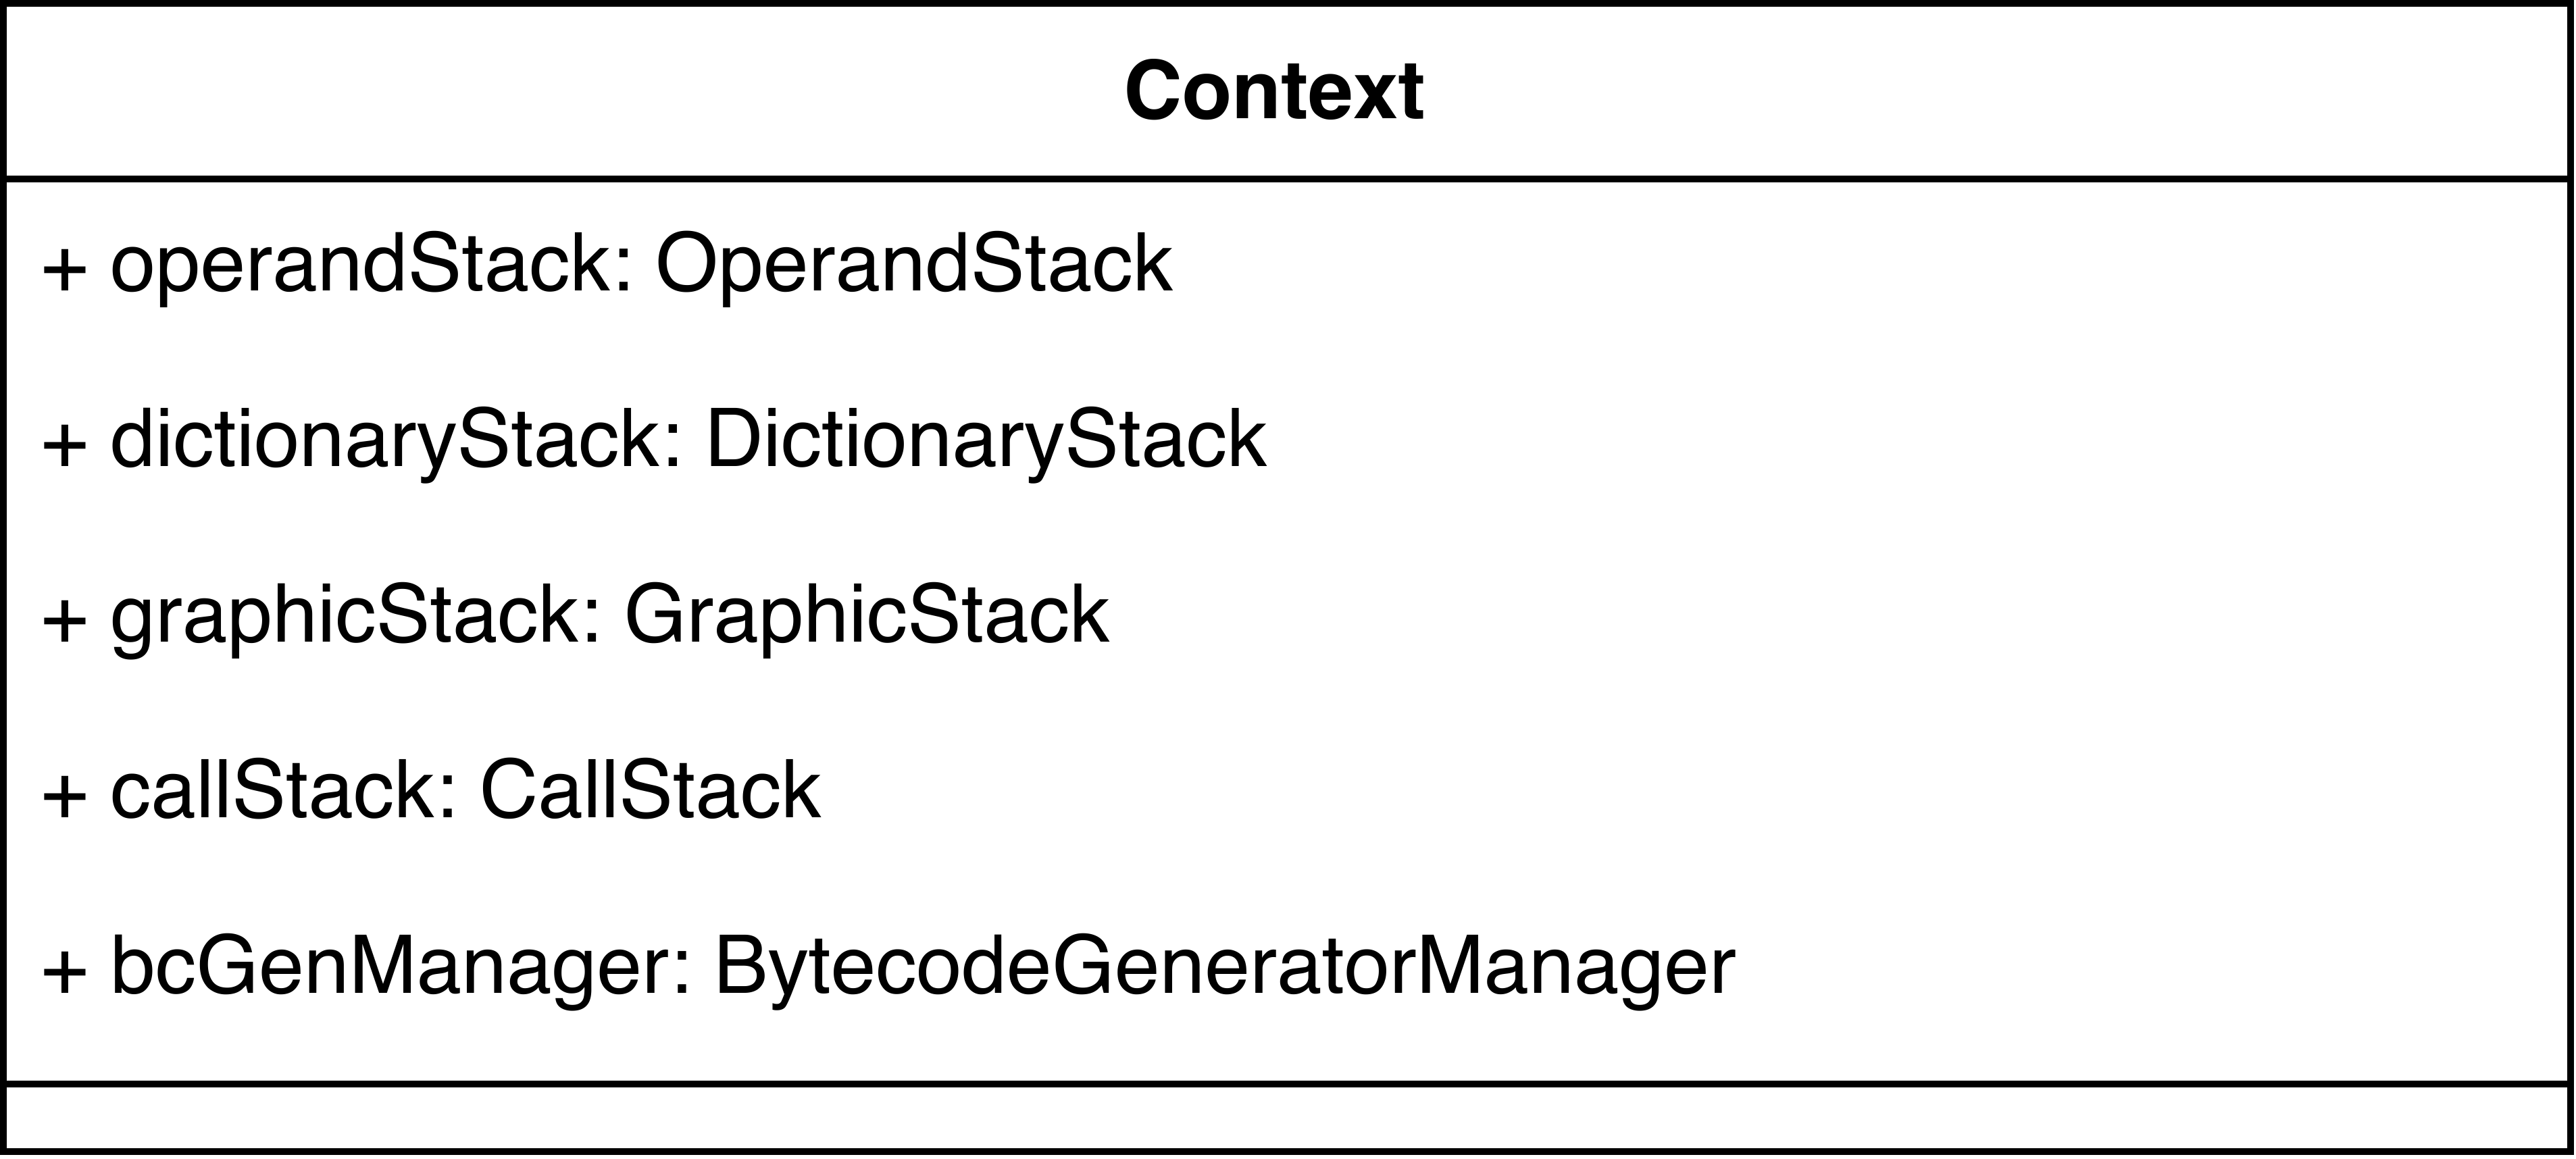
\includegraphics[width=0.8\linewidth]{Context.png}
	\caption{Класс Context}
\end{figure}


Если раньше все эти компоненты находились в библиотеке поддержке времени исполнения, то теперь они выделены в отдельную структуру. Таким образом, появилась возможность параллельного выполнения задач отрисовки с переключением между ними, а значит параллельной отрисовки интерфейса. 

Возможность параллельной обработки интерфейса была реализована с помощью использования очереди отрисовки, в которой хранятся операторы рисования, реализованные в классе \texttt{PSPrimitive}. Класс \texttt{PSPrimitive} объединяет в себе все рисующие операторы языка: операторы заливки, рисования линии и так далее. В этом классе также хранится текущий графический путь и ссылка на тот контекст, в котором производится исполнение, из которого берутся параметры и в который кладутся результаты работы.
Всё это позволило реализовать выполнение фоновых задач. В качестве примера были реализованы развороты диалогового окна по вертикали и горизонтали на 180 градусов, запуск волны по щелчку правой кнопкой мыши.

% У заключения нет номера главы
\section*{Заключение}
В ходе выполненной работы были достигнуты следующие результаты.
\begin{itemize}
\item Спроектирован механизм обработки событий.
\item Выполнено и реализовано расширение языка PostScript:
\begin{itemize}
    \item поддержка событий;
    \item обработчики событий мыши и клавиатуры;
    \item отладочные операторы.
\end{itemize}
\item Выполнена поддержка выполнения фоновых задач:
\begin{itemize}
    \item реализована очередь выполнения графических примитивов;
    \item реализована очередь выполнения событий;
    \item реализована многопоточность.
\end{itemize}
\end{itemize}

% \begin{figure}[h!]
%   \centering
%   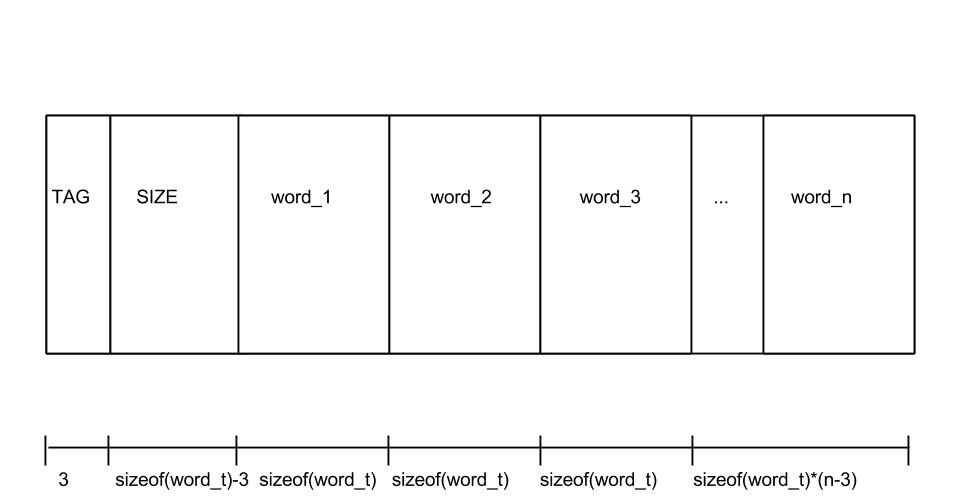
\includegraphics[]{1.gif}
% \end{figure}

% \bibliographystyle{unsrtnat}
 \bibliographystyle{unsrt}
%\bibliographystyle{ugost2008ls}
\bibliography{diploma.bib}
\end{document}


